% !TEX root = 00_arbeit.tex

%---------------------------------------------------------------------------------
%% Stata

\section{Analyse der Prognosefähigkeit}\label{sec:analyse}

Aufgrund der in \autoref{sec:vergleich_la} festgestellten Einflüsse auf die Vorhersagegenauigkeit eines Netzwerkes werden in diesem Abschnitt diese Faktoren variiert, um herauszufinden, welche Parameter zu einem Netzwerk mit geringster Prognoseabweichung führen. Hierzu werden die in \autoref{sec:algorithm} vorgestellten Algorithmen in Stata implementiert und mit einem gemeinsamen Datensatz untersucht. Die Ergebnisse dieser Untersuchung werden in diesem Abschnitt näher betrachtet. Zu diesem Zweck wird der eingesetzte Datensatz zunächst beschrieben. Nachfolgend werden die Vorbereitungen der Messungen erklärt. Anschließend erfolgen die Auswertungen der Prognosefähigkeit des Backpropagation-Verfahren und des Levenberg-Marquardt Algorithmus. Schließlich werden die Ergebnisse der Auswertung gegenübergestellt.

%In diesem Abschnitt erfolgt die Analyse der Prognosefähigkeit eines MLP-Netzwerkes. Hierbei werden die in \autoref{sec:algorithm} hergeleiteten Algorithmen einem Vergleich unterzogen.


\subsection{Erklärung des Datensatzes}\label{sec:datensatz}

%\farbig{Beide Lernalgorithmen werden im Hinblick auf ihre Lerngeschwindigkeit und ihr Vorhersagevermögen untersucht. Hierzu werden die, in \autoref{sec:algorithm} vorgestellten Algorithmen in Stata implementiert und mit Hilfe des, in \autoref{tab:datensatz} dargestellten, Datensatzes untersucht.} 
Der Datensatz besteht aus einer Zeitreihe der in \autoref{tab:datensatz} dargestellten Variablen. Dabei ist in der ersten Spalte die Variable des Datensatzes, nachfolgend die Einheiten, in den nächsten beiden Spalten der Minimal- und Maximalwert der Variable im betrachteten Zeitraum und in der letzten Spalte die Herkunft der Information dargestellt. Der betrachtete Zeitraum erstreckt sich vom 01.04.2010 bis zum 27.08.2016. Der Strompreis ist für jede Stunde eines jeden Tages angegeben und beinhaltet somit 56.180 Datenpunkte. Nicht jede Variable des Datensatzes besitzt in seiner ursprünglichen Form 24 Werte für einen Tag. In diesen Fällen werden die fehlenden Daten entweder extra- bzw. interpoliert, um die Anzahl der Daten an den Strompreis anzupassen. Außerdem werden die Variablen an dieselbe Währung angepasst. Für diesen Zweck wird der tägliche US-Dollar/Euro Wechselkurs genutzt, um den Kohlepreis von \$/Tonne, den Heizölpreis von \$/Gallone und den Uranpreis von \$/kg respektive in €/Tonne, €/Gallone und €/kg umzurechnen.

\begin{filecontents*}{datensatz.tex}
{\setstretch{1.0}
\captionsetup{skip=1pt,margin=5pt,position=below} %skip=1pt,
\rowcolors{3}{tableShade}{white}

\begin{longtable}{Zrccl}
    \caption[Überblick der untersuchten Variablen]{Auflistung einzelner Variablen des Datensatzes für die Untersuchung der Prognosefähigkeit.} \label{tab:datensatz}\\
    \toprule
    \hiderowcolors

        Variable                         & Einheit    & Minimalwert   & Maximalwert   & Quelle            \\
    \midrule
    \endfirsthead
        \multicolumn{5}{c}{\footnotesize \tablename\ \thetable{}: Fortsetzung der vorherigen Seite} \\
    \toprule
        %\multicolumn{1}{l}{\textbf{Verweis}} & \multicolumn{1}{Z}{\textbf{Modell}} & \multicolumn{1}{Z}{\textbf{Lernalgorithmus}} & \multicolumn{1}{Z}{\textbf{Markt}} & \multicolumn{1}{Z}{\textbf{Performancemaß}} \\
        Variable                         & Einheit    & Minimalwert   & Maximalwert   & Quelle            \\

    \midrule
    \endhead
    \midrule
        \multicolumn{5}{c}{{\footnotesize \tablename\ \thetable{}: Fortsetzung auf der nächsten Seite}} \\
    \bottomrule
    \endfoot
    \bottomrule
        \caption*{\footnotesize $^*$\,Internetseiten der Übertragungsbetreiber: Amprion, Tennet, 50Hertz, TransnetBW. Werte wurden aufsummiert. $^\dagger$\,Der Preis wurde von US-Dollar in Euro umgerechnet, fehlende Daten extra- bzw. interpoliert und der Tagespreis wurde für jede Stunde als konstant angenommen. }
        %\multicolumn{5}{c}{\footnotesize $^*$\,Internetseiten der Übertragungsbetreiber: Amprion, Tennet, 50Hertz, TransBW. Werte wurden aufsummiert. \farbig{\footnotesize Abkürzungen ausschreiben}}
        
    \endlastfoot
    \showrowcolors
        Strompreis                      & [€/MWh]       & $-221,99$ & $210$         & EEX.com           \\
        Erzeugte Energie aus Wind/Sonne & [MWh]         & $263,35$  & $44606,29$    & $^*$              \\
        Energieverbrauch                & [MWh]         & $29201$   & $79884$       & Entsoe.net        \\
        Kosten für CO$_2$               & [€/Tonne]     & $2,68$    & $16,84$       & EEX.com           \\
        Erdgaspreis                     & [€/MWh]       & $11,24$   & $29,06$       & Thomson Reuters   \\
        Kohlepreis$^\dagger$            & [€/Tonne]     & $47,995$  & $190,414$     & EEX.com           \\
        Heizölpreis$^\dagger$           & [€/Gallone]   & $0,941$   & $4,867$       & Thomson Reuters   \\
        Uranpreis$^\dagger$             & [€/kg]        & $81,028$  & $232,458$     & Thomson Reuters   \\
        Stunde des Tages                & [h]           & $1$       & $24$          & -                 \\
        Tag der Woche                   & [d]           & So:\,$0$  & Sa:\,$6$      & -                 \\
        
\end{longtable}

}
\end{filecontents*}
\LTXtable{\textwidth}{datensatz}

Der Datensatz bestehend aus 56.180 Datenpunkten wird pro Variable in zwei Sets unterteilt. Das Trainingsset beinhaltet 46.180 Datenpunkte und das Testset besteht aus 10.000 Datenpunkten. Diese Unterteilung ist notwendig, um die Netzwerke out-of-sample\footnote{Dies ist ein aus dem englischen ins deutsche übernommener Begriff und beteutet, dass das zu testende Modell mit Daten getestet wird welche es während dem Training nicht \glqq gesehen\grqq~hat. Bei guten Ergebnissen beweist das Modell damit seine Generalisierungsfähigkeit.} untersuchen zu können und so dem in \autoref{sec:vergleich_la} besprochenen, \glqq Auswendiglernen\grqq~vorzubeugen. Somit wird ein Netzwerk nach dem Training danach bewertet, wie es die Strompreise der nächsten 10.000 Stunden vorhersagen kann.

\begin{figure}[!htb]
    \centering
        %% Compiler: XeLaTeX

\makeatletter
\def\datafile{Daten/misc/autocorrelation.txt}
\makeatother


    \pgfplotsset{
        minor x tick num=1,
        minor y tick num=1,
        xlabel near ticks,
        xmin=-3, xmax=171,
        width=15cm, %\textwidth,
        height=6cm,
    }

\usepgfplotslibrary{statistics}

\begin{tikzpicture}
\begin{axis}[
    xlabel=Lag,
    ylabel=Autokorrelation,
    xtick       ={0,24,48,72,96,120,144,168},
    xmajorgrids=true,
    ymajorgrids=true,
    major grid style={line width=.2pt,draw=black!80,dotted},
]
\addplot [
    ycomb,
    restrict x to domain=0:171,
] 
table [
    x=lag, 
    y=AC, 
    /pgf/number format/read comma as period,
    col sep=tab,
] {\datafile};
\end{axis}
\end{tikzpicture}
    \caption{Autokorrelation der stündlichen Elektrizitätspreise.}
    \label{fig:autokorrelation}
\end{figure}

Bevor ein zukünftiger Strompreis anhand heute zur Verfügung stehender Daten vorhergesagt wird, ist es wichtig zu überlegen, welcher Vorhersagehorizont sinnvoll ist.
Zu diesem Zweck ist in \autoref{fig:autokorrelation} die Autokorrelation der Elektrizitätspreise dargestellt, wobei ein Lag (deutsch: Verschiebung) eine Stunde repräsentiert. Die Betrachtung der Autokorrelation ermöglicht es, eine Zeitreihe dahingehend zu untersuchen, ob und wie zwei Beobachtungen in Beziehung zueinander stehen. Je höher die Autokorrelation ist, desto höher ist auch die Abhängigkeit einer Beobachtung zum Zeitpunkt t$\neq$0 in Bezug auf die Beobachtung zum Zeitpunkt t$=$0. Diese Abhängigkeit wird auch als Korrelation bezeichnet. Der \autoref{fig:autokorrelation} kann entnommen werden, dass die Beobachtung mit einem Lag von Eins die höchste Korrelation aufweist. Zusätzlich bilden die Autokorrelationswerte im Abstand von 12 und 24 Stunden Maxima aus, wobei die Maxima im Abstand von 24 Stunden deutlich höhere Werte aufweisen als die Maxima der 12-stündigen Abstände. Daneben weisen die 24. und 168. Stunde die höchste Autokorrelation auf. 
Hieraus kann geschlossen werden, dass die vorherige Stunde den höchsten Informationsgehalt zur Vorhersage der betrachteten Stunde liefert. Unter der Berücksichtigung von \autoref{sec:vorhersagemodelle}, in dem erläutert wurde, dass der Strompreis durch den Marktbetreiber nicht einzeln für jede Stunde sondern für 24 Stunden eines nächsten Tages gebildet wird, ist ersichtlich, dass der Preis der vorherigen Stunde zum Zeitpunkt einer Vorhersage nicht zur Verfügung steht. Unter Realbedingungen ist es somit am erfolgversprechendsten, wenn die gleiche Stunde des vorherigen Tages oder der vergangenen Woche des gleichen Tages zur Vorhersage genutzt wird. In dieser Arbeit wird daher der 24 stündige Vorhersagehorizont für die nachfolgenden Untersuchungen gewählt.

\subsection{Vorbereitung der Messungen}

Die von der Netztopologie bedingten Faktoren sind die Aktivierungsfunktion, die An- bzw. Abwesenheit des Bias-Neurons und der Lernalgorithmus. Zusätzlich spielen bei dem Lernalgorithmus die jeweiligen Parameter eine Rolle, dessen optimale Werte bestimmt werden müssen, bevor die Prognosefähigkeit des Netzes bewertet werden kann.
Im Folgenden wird der Einfluss dieser Faktoren auf die Vorhersagegenauigkeit untersucht. Zum Einsatz kommt hierfür ein dreischichtiges MLP, welches in \autoref{fig:MLP-Algorithm} dargestellt ist. Wie in \autoref{sec:vergleich_la} erklärt, wird die Anzahl der Eingabeneuronen durch die Anzahl an Variablen bestimmt. Die in dieser Arbeit verwendeten Variablen werden in \autoref{sec:datensatz} näher beschrieben. Die optimale Anzahl der verdeckten Neuronen wird iterativ bestimmt und da der Strompereis prognostiziert werden soll, beträgt die Anzahl an Ausgabeneuronen 1. 

Als Aktivierungsfunktion werden die logistische Funktion und der Tangens-Hyperbolicus untersucht. Da der Wertebereich der logistischen Funktion [0,1] und der Wertebereich des Tangens-Hyperbolicus [-1,1] beträgt, werden alle Variablen des Datensatzes auf diese Wertebereiche angepasst. Zu diesem Zweck wird die Min-Max bzw. die lineare Normalisierung
\begin{equation}
x_i'=(max_{Ziel} - min_{Ziel}) \cdot \left ( \frac{x_i-min_{Daten}}{max_{Daten}-min_{Daten}} \right ) + min_{Ziel}
\label{gl:norm}
\end{equation}
mit $x_i$ als Ausgangswert, $x_i'$ als normalisierter Wert, $max_{Ziel}$/$min_{Ziel}$ als Maximal-/Minimalwert des gewünschten Wertebereiches und $max_{Daten}$/$min_{Daten}$ als Maximal-/Minimalwert der Variable im betrachteten Zeitraum durchgeführt. Der Vorteil dieses Normalisierungsverfahrens liegt darin, dass die Proportionen der Daten im neuen Wertebereich erhalten bleiben. Somit bleiben auch die Abhängigkeiten und Beziehungen zwischen den Variablen erhalten.\,\citef[16]{neuralnet_intro} 

Betrachtet man die logistische Funktion, so werden die Werte 0 bzw. 1 asymptotisch in der Unendlichkeit erreicht. Somit lernt das Netzwerk bei der Eingabe der beiden Werte nur sehr langsam.\,\citef[158]{Rashid2016} Aus diesem Grund wird der Datensatz auf den Wertebereich [0.1,0.9] geändert. Die gleiche Begründung führt beim Tangens-Hyperbolicus zu einem Wertebereich von [-0.9,0.9].

Um die Einflüsse der in \autoref{sec:vergleich_la} besprochenen \glqq schlechten\grqq~Minima zu reduzieren, werden in dieser Arbeit 20 Neuinitialisierungen durchgeführt, um die optimalen Parameter zu finden.

Mit der Variation des Lernalgorithmus, der Aktivierungsfunktion und der An- und Abwesenheit des Bias-Neurons ergeben sich acht Variationsmöglichkeiten, bei denen zunächst aus der Begründung aus \autoref{sec:eval_maße} folgernd mit Hilfe des $RMSE$ die optimalen Netzparameter bestimmt werden. Das Optimum eines Parameters ist erreicht, wenn die Abweichung zwischen vorhergesagtem und tatsächlichen Preis am geringsten ist und somit den niedrigsten $RMSE$ aufweist. Anschließend wird die Vorhersagegenauigkeit eines jeden Lernalgorithmus mit den jeweiligen optimalen Parametern wie in \autoref{sec:eval_maße} erläutert mit Hilfe des $RMSE$, $MAE$, $ABS$, $REL$, $R^2$, $RAE$, $MAPE_2$ und des $sMAPE$ ausgewertet.




\subsection{Auswertung der Prognosefähigkeit des Backpropagation-Verfahrens}\label{sec:aus_backprop}

Bei dem klassischen Backpropagation-Verfahren, welches in \autoref{sec:Backpropagation} vorgestellt wird, wird zunächst die optimale Lernrate $\alpha$ bestimmt. Anschließend wird die passende Anzahl an verdeckten Neuronen ermittelt und schließlich wird die vertretbare Anzahl an Epochen festgelegt.

Hierzu wird in \autoref{fig:BP_logist_o_lrate} zunächst anhand eines MLP mit logistischer Aktivierungsfunktion und ohne Bias-Neuron beispielhaft gezeigt wie die optimale Lernrate in dieser Arbeit ermittelt wird. Zunächst wird die Anzahl der verdeckten Neuronen im einstelligen Bereich eingestellt. In diesem Falle sind es 5 verdeckte Neuronen. Als nächstes wird die Lernrate von 0 bis 1 in einer Schrittweite von 0,001 erhöht und das Netzwerk wird bei jedem Schritt 20 Mal neu initialisiert, trainiert und mit dem Testset getestet. So entstehen 20 $RMSE$-Werte, die anschließend gemittelt werden und in \autoref{fig:BP_logist_o_lrate} im oberen Graphen aufgetragen werden. Dieser weist gerade zu Beginn zwar ein Minimum auf aber durch die Sprunghaften Änderungen, die auf \glqq schlechte\grqq~Minima der Fehlerlandschaft zurückzuführen sind, erweist sich die Bestimmung des $RMSE$-Minimums mit dem bloßen Auge als problematisch. Durch den konkaven Verlauf des Graphen hat auch das Fitten der Daten mit den Standardfunktionen in OriginLab zu keinem zufriedenstellenden Ergebnis geführt.

\begin{figure}[!htb]
    \centering
        
\makeatletter
\def\datafilea{Daten/BP/logist/o/BP_logis_o-lernrate_0-1_0,001.txt}
\def\datafileb{Daten/BP/logist/o/BP_logis_o-lernrate_0-0,2_0,0002.txt}
\makeatother

    \pgfplotsset{
        xticklabel style={
            /pgf/number format/precision=3,
            /pgf/number format/fixed},
    }


%%-------------------Lernrate-BP-logis-o---------------------%%


\begin{tikzpicture}
\def\x{l_rate}
\def\y{RMSE}
\def\xname{Lernrate}
\def\yname{\y}
 \begin{groupplot}[
        group style = {group size = 1 by 2},
        height = 6cm,
        width = 15cm,
        ylabel=\yname,
        minor x tick num=1,
        minor y tick num=1,
    ]
%%----------------------RMSE-0_1-----------------------------%%
    \nextgroupplot[
        xmin=-0.015,
        xmax=1.015,
    ]
 
    \addplot[
        mark=none,
        draw=black,
    ] 
    table[
        skip coords between index={0}{1},
        /pgf/number format/read comma as period,
        x=\x, 
        y=\y_mean, 
        col sep=tab,
    ] {\datafilea};
    
    \draw[blue, dashed, line width=1pt] (axis cs:-0.015,0) rectangle (axis cs:0.2,30);
    \coordinate (top) at (rel axis cs:0,0);
    \coordinate (top-) at (rel axis cs:0.208,0);
%%----------------------RMSE-0_0,2-----------------------------%%
    \nextgroupplot[
        xlabel=\xname,
        xmin=-0.005,
        xmax=.2005,
    ]
 
    \addplot[
        mark=none,
        draw=black,
    ] 
    table[
        skip coords between index={0}{3},
        /pgf/number format/read comma as period,
        x=\x, 
        y=\y_mean, 
        col sep=tab,
    ] {\datafileb};
    \addlegendentry{Messung}
    
    \addplot[
        line width=1pt,
        mark=none,
        draw=red,
        domain=0.0006:0.2,
        samples=401, 
        unbounded coords=discard,
    ] {((1.13588E-8)*x^2+(9.75296E-9)*x + (1.13103E-11))/((7.22463E-10)*x+(1.44668E-13))};
    \addlegendentry{Fit}
    \coordinate (bot) at (axis cs:-0.005,31.5);
    \coordinate (bot-) at (axis cs:0.2,31.5);

\end{groupplot}
\draw[blue, dashed, line width=1pt] (top) -- (bot);
\draw[blue, dashed, line width=1pt] (top-) -- (bot-);

\end{tikzpicture}
    \caption[Beispiel zur Bestimmung der Lernrate $\alpha$ beim BP-Verf.]{Bestimmung der Lernrate $\alpha$ mit dem geringsten Fehler bei einem MLP ohne Bias-Neuron, welches mit dem Backpropagation-Verfahren trainiert wird. Der untere Graph zeigt einen vergrößerten Ausschnitt des oberen Graphen.}
    \label{fig:BP_logist_o_lrate}
\end{figure}

Aus diesem Grund wird nochmals eine höher auflösende Messung im Bereich von 0 und 0,2 mit einer Schrittweite von 0,0002 durchgeführt, die in \autoref{fig:BP_logist_o_lrate} unten dargestellt ist. Der sich so ergebende Verlauf lässt sich durch eine schiefe Asymptote annähern, die in \autoref{fig:BP_logist_o_lrate} unten in rot abgebildet ist. Durch die erste Ableitung der angenäherten Funktion, lässt sich auch das $RMSE$-Minimum bei einer Lernrate von 0,025 bestimmen.\\


\begin{figure}[!htb]
    \centering
        \makeatletter
\def\datafile{Daten/BP/logist/o/BP_logis_o-hneuron.txt}
\makeatother

    \pgfplotsset{
        minor x tick num=1,
        minor y tick num=1,
        xmin=0, xmax=41,
        width=15cm, %\textwidth,
        height=6cm,
        %ylabel style={rotate=180},
        xticklabel style={
            /pgf/number format/precision=3,
            /pgf/number format/fixed},
    }

\begin{tikzpicture}
\def\x{h_neuron}
\def\y{RMSE}
\def\xname{Anzahl verdeckter Neuronen}
\def\yname{\y}
\begin{axis}[
    xlabel=\xname,
    ylabel=\yname,
    ]
 
    \addplot[
    mark=none,
    draw=black,
    ] 
    table[
    skip coords between index={40}{41},
    /pgf/number format/read comma as period,
    x=\x, 
    y=\y_mean, 
    col sep=tab,
    ] {\datafile};
    
\end{axis}
\end{tikzpicture}
    \caption[Beispiel zur Bestimmung der Anzahl verdeckter Neuronen beim BP]{Bestimmung der Anzahl an verdeckten Neuronen mit dem geringsten Fehler bei einem MLP der logistischen Funktion als Aktivierungsfunktion und ohne Bias-Neuronen. Der Graph zeigt pro Datenpunkt den Mittelwert aus 20 Einzelmessungen.}
    \label{fig:BP_logist_o_hneuron}
\end{figure}

Im nächsten Schritt wird die Anzahl der verdeckten Neuronen ermittelt. Dabei wird die Lernrate auf den zuvor bestimmten Wert eingestellt und die Anzahl der verdeckten Neuronen von 1 an um ein Neuron erhöht. Die Grenze hierbei wird nur durch die Rechenkapazität des Computers bestimmt, auf dem das Netzwerk berechnet wird. Wie aber in \autoref{sec:vergleich_la} festgestellt, tendiert ein Netzwerk mit steigender Anzahl an verdeckten Neuronen zum Auswendiglernen der Daten. Daher ist eine niedrige Anzahl zu bevorzugen. In dem gleichen Netzwerk, in dem die Lernrate bestimmt wird, kann der $RMSE$-Verlauf in Abhängigkeit der Anzahl verdeckter Neuronen in \autoref{fig:BP_logist_o_hneuron} eingesehen werden. Der niedrigste $RMSE$-Wert wird hier bei Drei verdeckten Neuronen gemessen.%\\ 

\begin{figure}[!htb]
    \centering
        

\colorlet{shadecolor}{gray!40}

\makeatletter
\def\datafile{Daten/BP/logist/o/BP_logis_o-epochen.txt}
\makeatother

    \pgfplotsset{
        minor x tick num=1,
        minor y tick num=1,
        xmin=0, xmax=51,
        width=15cm, %\textwidth,
        height=6cm,
        %ylabel style={rotate=180},
        xticklabel style={
            /pgf/number format/precision=3,
            /pgf/number format/fixed},
    }


%%----------------------RMSE-epochen-----------------------%%
\begin{tikzpicture}
\def\x{epochs}
\def\y{RMSE}
\def\xname{Epochen}
\def\yname{\y}
\begin{axis}[
    xlabel=\xname,
    ylabel=\yname,
    ]
 
    \addplot[
    mark=none,
    draw=black,
    ] 
    table[
    skip coords between index={40}{41},
    /pgf/number format/read comma as period,
    x=\x, 
    y=\y_mean, 
    col sep=tab,
    ] {\datafile};
    
    \addplot[
    name path=min,
    mark=none,
    draw=shadecolor,
    %domain=-0.01:1.01,    
    ] 
    table[
    /pgf/number format/read comma as period,
    x=\x, 
    y=RMSE_min, 
    col sep=tab,
    ] {\datafile};
    
    \addplot[
    name path=max,
    mark=none,
    draw=shadecolor,
    %domain=-0.01:1.01,    
    ] 
    table[
    /pgf/number format/read comma as period,
    x=\x, 
    y=RMSE_max, 
    col sep=tab,
    ] {\datafile};
    
    \addplot [shadecolor] fill between[ 
    of = min and max,
    ];
    
\end{axis}
\end{tikzpicture}
    \caption[Beispiel zur Bestimmung der Anzahl an Epochen]{Bestimmung der der Anzahl an vertretbarer Epochen, wobei die graue Fläche den jeweiligen Maximal- bzw. Minimalwert einer Messung und der schwarze Graph den Mittelwert darstellt.}
    \label{fig:BP_logis_o_epochen}
\end{figure}

Schließlich wird die Anzahl der Epochen bestimmt, in dem die Lernrate auf 0,025 und die Anzahl an verdeckten Neuronen auf Drei gesetzt wird und die Epochenanzahl von Eins an, um eine Epoche erhöht wird. Das Ergebnis dieser Messung ist in \autoref{fig:BP_logis_o_epochen} dargestellt. Hierbei gibt die graue Fläche den jeweiligen Maximal- bzw. Minimalwert einer Messung an und der schwarze Verlauf den Mittelwert. Gerade an dem Maximalwert lässt sich erkennen, dass die Höhe der Fehler mit steigender Epochenanzahl geringer wird und ab 30 Epochen auch die Höhe der Ausreißer sprunghaft abnimmt. Der Minimalwert hingegen bewegt sich durchgehend zwischen 8 und 9. Daraus kann geschlossen werden, dass mit steigender Anzahl an Epochen die Wahrscheinlichkeit steigt, bessere Minima zu erreichen oder das Netzwerk anfängt die Daten auswendig zu lernen. Dies wurde zwar versucht durch den geteilten Datensatz zu vermeiden, dennoch wird in der Literatur\,\citef[60]{dkriesel07} darauf hingewiesen, dass wenn das Testset dazu benutzt wird, um die optimalen Parameter eines Netzwerkes zu bestimmen, das Netzwerk so auch auf die Testdaten zugeschnitten wird. Um hier Abhilfe zu schaffen, wird empfohlen ein drittes Validierungsset zu erstellen\,\citef[44]{neuralnet_intro}, welches nur der Evaluation des Netzes dient oder es wird bewusst eine geringere Anzahl an Epochen gewählt. In dieser Arbeit kommt die letztere Methode zur Anwendung. Somit wird, für das MLP mit logistischer Aktivierungsfunktion und ohne Bias-Neuron, eine Epochenanzahl von 30 gewählt. Da ab diesem Wert eine deutliche Veränderung des $RMSE$-Verlaufes zu beobachten ist.

Bei der Bestimmung der optimalen Parameter der Netzwerke, welche sich in der Aktivierungsfunktion und dem Vorhandensein eines Bias-Neurons unterscheiden, wird analog vorgegangen.
In \autoref{tab:BP_resultat} ist das Ergebnis der Untersuchung dargestellt. Dabei ist links zunächst die genutzte Aktivierungsfunktion aufgeführt. Nachfolgend ist dargestellt ob das Netzwerk ein Bias-Neuron besitzt oder nicht, wobei \glqq m\grqq~für mit und \glqq o\grqq~für ohne Bias-Neuron steht. Als nächstes werden die optimalen Werte für die Lernrate, Anzahl der verdeckten Neuronen und Anzahl der Epochen genannt. Darauf folgend wird die Zeit angegeben, die für das Bestimmen der optimalen Parameter benötigt wird. Hierfür wurden die Dauer der einzelnen Messungen, zur Bestimmung der optimalen Parameter, aufsummiert. An dieser Stelle wird darauf hingewiesen, dass die Optimierungszeit für das Netzwerk mit dem Tangens-Hyperbolicus als Aktivierungsfunktion geringer ist, da bei der Bestimmung der optimalen Lernrate die Messung von 0 bis 1 in einer Schrittweite von 0,001 ausgereicht hat. Um die Vergleichbarkeit der Daten zu gewährleisten, wurden die Messungen für jede Netzwerkkonstellation bis zur 50. Epoche und bis zum 40. verdeckten Neuron durchgeführt. Schließlich wurden, mit den optimalen Parametern eines jeden Netzwerkes, 20 Vorhersagen mit dem Testset erstellt und das beste Ergebnis in Form des kleinsten $RMSE$ (aufgeführt als min. $RMSE$) ermittelt. Die Berechnungszeit gibt abschließend die Zeit an die das Netzwerk gebraucht hat, um trainiert zu werden und die Prognose mit dem aufgeführten $RMSE$-Wert zu erstellen. 


%\newpage

\begin{filecontents*}{BP_resultat.tex}
{\setstretch{1.0}
\captionsetup{skip=1pt,margin=5pt,position=below} %skip=1pt,
\rowcolors{3}{tableShade}{white}

\begin{longtable}{cccccccc}
    %\captionsetup{justification=centering}
    \caption[Optimale Parameter und die erreichte Prognosegenauigkeit des BP-Verf.]{Optimale Parameter und die erreichte Prognosegenauigkeit, in Form des $RMSE$-Wertes, des BP-Verfahrens.} \label{tab:BP_resultat}\\
    \toprule
    \hiderowcolors

       \multicolumn{1}{Y}{Aktivierungs funktion} &      \multicolumn{1}{Y}{Bias- Neuron} &   \multicolumn{1}{Y}{Lern- rate} &  \multicolumn{1}{Y}{verd. Neuronen} &  \multicolumn{1}{Y}{Epochen} &  \multicolumn{1}{Y}{Optimierungs zeit} & \multicolumn{1}{Y}{min. $RMSE$}  & \multicolumn{1}{Y}{Berechnungs zeit} \\

    \midrule
    \endfirsthead
        \multicolumn{8}{c}{\footnotesize \tablename\ \thetable{}: Fortsetzung der vorherigen Seite} \\
    \toprule
       \multicolumn{1}{Y}{Aktivierungs funktion} &      \multicolumn{1}{Y}{Bias- Neuron} &   \multicolumn{1}{Y}{Lern- rate} &  \multicolumn{1}{Y}{verd. Neuronen} &  \multicolumn{1}{Y}{Epochen} &  \multicolumn{1}{Y}{Optimierungs zeit} & \multicolumn{1}{Y}{min. $RMSE$}  & \multicolumn{1}{Y}{Berechnungs zeit} \\
    \midrule
    \endhead
    \midrule
        \multicolumn{8}{c}{{\footnotesize \tablename\ \thetable{}: Fortsetzung auf der nächsten Seite}} \\
    \bottomrule
    \endfoot
    \bottomrule
        \caption*{\footnotesize logist.: logistische Funktion, Tanh.: Tangens-Hyperbolicus, o: ohne Bias-Neuronen, m: mit Bias-Neuronen}

        
    \endlastfoot
    \showrowcolors
        logist.                 & o       & 0,025 & 3         & 30  & 7h:44m:39s & 8,31 & 10s         \\
        logist.                 & m       & 0,016 & 3         & 33  & 8h:44m:11s & 8,95 & 15s         \\
        Tanh.                   & o       & 0,81  & 5         & 30  & 6h:46m:50s & 9,24 & 14s         \\
        Tanh.                   & m       & 0,83  & 5         & 27  & 8h:29m:29s & 9,83 & 16s         \\

        
\end{longtable}

}
\end{filecontents*}
\LTXtable{\textwidth}{BP_resultat}

Aus der \autoref{tab:BP_resultat} folgt, dass die Lernrate und die optimale Anzahl verdeckter Neuronen von der Aktivierungsfunktion abhängen. Die An- oder Abwesenheit von Bias-Neuronen beeinflusst diese Faktoren jedoch nicht. Die optimale Anzahl an Epochen liegt durchgehend in der Nähe von 30 und ist somit in Gänze unabhängig von den anderen Parametern. Durch die abweichende Herangehensweise bei der Bestimmung der Lernrate, können die Optimierungszeiten der Aktivierungsfunktionen nicht direkt verglichen werden. Bei gleicher Aktivierungsfunktion führt das Vorhandensein von Bias-Neuronen jedoch zu längeren Optimierungszeiten, wobei der Unterschied bei gleichen Bedingungen mehr als eineinhalb Stunden betragen kann. Auch die längere Berechnungszeit mit Bias-Neuronen deutet auf diese Abhängigkeit hin. Die Unterschiede in dem $RMSE$-Wert liegen im niedrigen einstelligen Bereich und sind damit nicht groß. Diese sind daher auf ungünstige Minima in der Fehlerlandschaft statt auf die Parameter des Netzwerkes zurückzuführen. Schließlich weist das Netzwerk mit logistischer Aktivierungsfunktion und ohne Bias-Neuronen die kleinste Abweichung in der Vorhersage über 10.000 Werte auf und wird daher im nächsten Schritt zur Bewertung der Vorhersagegenauigkeit näher betrachtet.

In \autoref{fig:BP_logis_o_result} ist nun der tatsächliche und der vorhergesagte Preis dargestellt. Der Übersichtlichkeit halber wurden die ersten und letzten 1.000 Werte im unteren Graphen aufgetragen. Dabei entsprechen 1.000 Stunden circa sechs Wochen. Die vier Graphen im oberen Bereich der Abbildung stellen Teilausschnitte des Gesamtverlaufes dar, die im unteren Graphen mit roten gestrichelten Linien umrandet sind. Für die weiteren Erläuterungen dient der obere linke Graph als Bezugspunkt, der nachfolgend als 1. Graph bezeichnet wird.


%\todo{In der fertigen Version den Graphen mit |input anstatt |includestandalone erzeugen. Da sonst die Schrift falsch dargestellt wird}

\begin{figure}[!htb]
    \centering
        %\includestandalone[mode=build,width=\textwidth]{Bilder/Plot/BP/BP_logis_o_result}
        %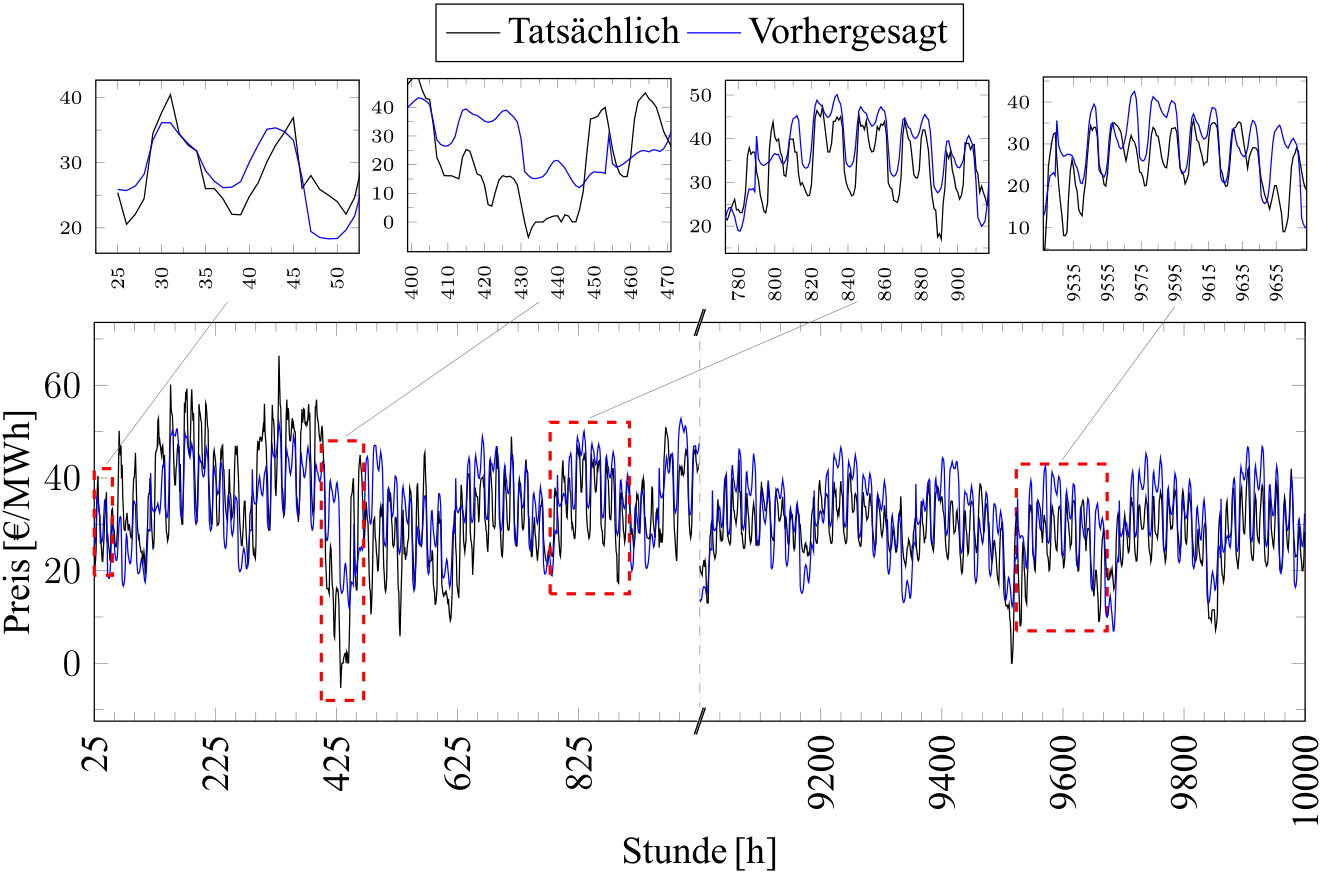
\includegraphics[width=0.92\textwidth]{Bilder/Plot/BP/BP_Preis.PNG}
        %%-------------------------------------------------------------------------
%% Quellen:
%% Discontinuity: http://www.yesterdayscoffee.de/tag/tikz/
%% https://tex.stackexchange.com/questions/149081/collapse-range-in-x-axis-with-pgfplots-break-x-axis
%% http://guido.vonrudorff.de/pgfplots-discontinuities/

\makeatletter
\def\datafile{Daten/BP/logist/o/BP_logis_result.txt}
\makeatother

    \pgfplotsset{
        minor x tick num=5,
        minor y tick num=1,
        x label style={yshift=.5em},
        y label style={yshift=-.5em},
        width=15cm, %\textwidth,
        height=6cm,
        xticklabel style={
            rotate=90,
        },
        every axis legend/.append style={
        at={(0.5,1.03)},
        anchor=south},
    }

%%----------------------result-----------------------%%
\begin{tikzpicture}
\begin{axis}[
    ylabel={Preis\,[€/MWh]},
    xlabel={Stunde\,[h]},
    xmin=25,
    xmax=2025,
    clip=false,
    xticklabels ={25,225,425,625,825,,9200,9400,9600,9800,10000},
    xtick       ={25,225,425,625,825,1025,1225,1425,1625,1825,2025},
    extra x ticks={1025},
    extra x tick style={grid=major, tick style={white, ultra thick}, tick label style={xshift=0cm,yshift=.30cm,rotate=90,}},
    extra x tick labels={\color{white}{/}},
    legend style={at={(.5,1.8)},anchor=north},
    legend columns=-1,
    ]

\addplot [mark=none,draw=black,restrict x to domain=25:1024,] 
table[
    x=index,
    y=real,
    col sep=tab,
    /pgf/number format/read comma as period,
] {\datafile};
\addlegendentry{Tats\"achlich}

\coordinate (unten) at (axis cs:1025,-12.5);
\coordinate (oben) at (axis cs:1025,73.5);
\draw[white, dashed, line width=.5pt] (unten) -- (oben);

\addplot [mark=none,blue,restrict x to domain=25:1024,] 
table[
    x=index,
    y=predict,
    col sep=tab,
    /pgf/number format/read comma as period,
] {\datafile};
\addlegendentry{Vorhergesagt}

\coordinate (oben1) at (axis cs:245,103);
%\coordinate (oben1) at (axis cs:55,50);
\draw[red, dashed, line width=1pt] (axis cs:25,19) rectangle (axis cs:55,42);
\draw[gray, line width=.2pt] (axis cs:45,43) -- (axis cs:245,80);

\coordinate (oben2) at (axis cs:760,102);
%\coordinate (oben2) at (axis cs:425,40);
\draw[red, dashed, line width=1pt] (axis cs:400,-8) rectangle (axis cs:470,48);
\draw[gray, line width=.2pt] (axis cs:440,49) -- (axis cs:760,80);

\coordinate (oben3) at (axis cs:1285,102);
%\coordinate (oben3) at (axis cs:825,50);
\draw[red, dashed, line width=1pt] (axis cs:778,15) rectangle (axis cs:909,52);
\draw[gray, line width=.2pt] (axis cs:844,53) -- (axis cs:1285,79);

\coordinate (oben4) at (axis cs:1810,100);
%\coordinate (oben4) at (axis cs:1625,45);
\draw[red, dashed, line width=1pt] (axis cs:1548,7) rectangle (axis cs:1698,43);
\draw[gray, line width=.2pt] (axis cs:1624,44) -- (axis cs:1810,75);

\addplot [mark=none,draw=black,restrict x to domain=1025:2024,] 
table[
    x=index,
    y=real,
    col sep=tab,
    /pgf/number format/read comma as period,
] {\datafile};

\addplot [mark=none,blue,restrict x to domain=1025:2024,] 
table[
    x=index,
    y=predict,
    col sep=tab,
    /pgf/number format/read comma as period,
] {\datafile};

\end{axis}
\node at (unten)[white,thick] {/};
\node at (unten) {/\!\!/};
\node at (oben)[white,thick] {/};
\node at (oben) {/\!\!/};

\node at (oben1) {%
    \begin{tikzpicture}[baseline,trim axis left,trim axis right]
    \begin{axis}[
      tiny,
      width=4.5cm, height=3.5cm,
      minor x tick num=1,
      minor y tick num=1,
      xmin=25,xmax=50,
      ytick       ={20,30,40},
      enlargelimits,
    ]
    \addplot +[mark=none,black,] table [x=index,y=real,col sep=tab,/pgf/number format/read comma as period,] {\datafile};
    \addplot +[mark=none,blue,] table [x=index,y=predict,col sep=tab,/pgf/number format/read comma as period,] {\datafile};
    \end{axis}
    \end{tikzpicture}%
    };

\node at (oben2) {%
    \begin{tikzpicture}[baseline,trim axis left,trim axis right]
    \begin{axis}[
      tiny,
      width=4.5cm, height=3.5cm,
      minor x tick num=1,
      minor y tick num=1,
      xmin=405,xmax=465,
      ytick       ={0,10,20,30,40},
      enlargelimits,
    ]
    \addplot +[mark=none,black,] table [x=index,y=real,col sep=tab,/pgf/number format/read comma as period,] {\datafile};
    \addplot +[mark=none,blue,] table [x=index,y=predict,col sep=tab,/pgf/number format/read comma as period,] {\datafile};
    \end{axis}
    \end{tikzpicture}%
    };

\node at (oben3) {%
    \begin{tikzpicture}[baseline,trim axis left,trim axis right]
    \begin{axis}[
      tiny,
      width=4.5cm, height=3.5cm,
      minor x tick num=1,
      minor y tick num=2,
      xmin=785,xmax=905,
      enlargelimits,
    ]
    \addplot +[mark=none,black,] table [x=index,y=real,col sep=tab,/pgf/number format/read comma as period,] {\datafile};
    \addplot +[mark=none,blue,] table [x=index,y=predict,col sep=tab,/pgf/number format/read comma as period,] {\datafile};
    \end{axis}
    \end{tikzpicture}%
    };

\node at (oben4) {%
    \begin{tikzpicture}[baseline,trim axis left,trim axis right]
    \begin{axis}[
      tiny,
      width=4.5cm, height=3.5cm,
      minor x tick num=1,
      minor y tick num=1,
      xticklabels ={9535,9555,9575,9595,9615,9635,9655},
      xtick       ={1560,1580,1600,1620,1640,1660,1680},
      xmin=1555,xmax=1685,
      enlargelimits,
    ]
    \addplot +[mark=none,black,] table [x=index,y=real,col sep=tab,/pgf/number format/read comma as period,] {\datafile};
    \addplot +[mark=none,blue,] table [x=index,y=predict,col sep=tab,/pgf/number format/read comma as period,] {\datafile};
    \end{axis}
    \end{tikzpicture}%
    };
\end{tikzpicture}
    \caption[Gegenüberstellung des tatsächlichen und des vorhergesagten Preises beim BP]{Gegenüberstellung des tatsächlichen und des vorhergesagten Preises, unter Anwendung des Backpropagation-Verfahren. Dargestellt ist das MLP mit logistischer Aktivierungsfunktion, ohne Bias-Neuronen und einem $RMSE$-Wert von 8,31.}
    \label{fig:BP_logis_o_result}
\end{figure}

Bemerkenswert ist, dass gerade zu Beginn des Testsets die Vorhersage sehr nah an den tatsächlichen Wert kommt. Dies ist an der Darstellung der ersten 50 Stunden im 1. Grafen zu erkennen. Hier beträgt die maximale Abweichung bei der Vorhersage der ersten 50 Stunden circa 8 €/MWh. Dies kann durch die Unterteilung des gesamten Datensatzes in Trainings- und Testset begründet sein, da die letzten Datenpunkte des Trainingssets direkt an die ersten Datenpunkte des Testsets anknüpfen und so das Netzwerk in den ersten Stunden des Testsets über \glqq gelernte\grqq~Vorinformationen verfügt.
Bei einem gemäßigten Wochenverlauf folgt der vorhergesagte Preis gerade in den ersten 1.000 Stunden annähernd dem tatsächlichen Preis, was im 3. Graphen zu erkennen ist. Schwierigkeiten hat das Netzwerk aber bei der Vorhersage von Spitzen-Werten. Dies lässt sich durchgehend beobachten und in dem 2. Graphen wird dies sehr deutlich. Hier beträgt die Abweichung bis zu 25 €/MWh und der Verlauf der vorhergesagten Werte folgt nur annähernd den tatsächlichen Werten. Abschließend lässt sich im 4. Graphen erkennen, dass gegen Ende des Testsets die lokalen Wochenminima zwar kleinere Abweichungen zeigen aber die Vorhersage, im Vergleich zu den ersten 1.000 Stunden, eine größere Überschätzung aufweist.

Abschließend erfolgt die Bewertung des Vorhersagevermögens des Netzwerkes anhand der zuvor ausgewählten Performancemaße. Diese sind in \autoref{tab:BP_schaetzer} aufgeführt.

%\todo{EV und U2 werden gestrichen.}

\begin{filecontents*}{BP_resultat.tex}
{\setstretch{1.0}
\captionsetup{skip=1pt,margin=5pt,position=below} %skip=1pt,
\rowcolors{3}{tableShade}{white}

\begin{longtable}{cccccccc}
    %\captionsetup{justification=centering}
    \caption[Übersicht der Performancemaße des genauesten Netzwerkes beim BP-Verf.]{Übersicht der Performancemaße des MLP mit logistischer Aktivierungsfunktion und ohne Bias-Neuronen.} \label{tab:BP_schaetzer}\\
    \toprule
    \hiderowcolors
        $RMSE$ & $MAE$ & $ABS$ & $REL$ & $R^2$ & $RAE$ & $MAPE_2$ & $sMAPE$ \\
    \midrule
    \endfirsthead
        \multicolumn{8}{c}{\footnotesize \tablename\ \thetable{}: Fortsetzung der vorherigen Seite} \\
    \toprule
        $RMSE$ & $MAE$ & $ABS$ & $REL$ & $R^2$ & $RAE$ & $MAPE_2$ & $sMAPE$ \\
    \midrule
    \endhead
    \midrule
        \multicolumn{8}{c}{{\footnotesize \tablename\ \thetable{}: Fortsetzung auf der nächsten Seite}} \\
    \bottomrule
    \endfoot
    \bottomrule
    \endlastfoot
    \showrowcolors
        8,307 & 6,18 & -0,421 & -0,015 & 0,754 & 43,929 & 21,597 & 26,041 \\
\end{longtable}

}
\end{filecontents*}
\LTXtable{\textwidth}{BP_resultat}

\newpage

Das $R^2$ besitzt mit 0,754 einen positiven Wert der näher an der 1 als an 0,5 ist und der $RAE$-Wert ist mit 43,929 deutlich unter 100. Hiermit weist das Netzwerk eine höhere Vorhersagegenauigkeit auf, als der historische Mittelwert. Das $ABS$ und $REL$ weisen beide einen negativen Wert auf, was auf eine Unterschätzung bei der Gesamtvorhersage hindeutet. Das $RMSE$ und das $MAE$ weisen bei kleinen Werten auf eine gute Vorhersage hin. Die gleiche Aussage trifft auch auf das $MAPE_2$ und $sMAPE$ zu. Diese vier Maße liefern aber erst bei einem Vergleich eine Auskunft darüber, welche Methode eine bessere Vorhersage liefert. Dieser Vergleich wird nach der Auswertung des Levenberg-Marquardt Algorithmus durchgeführt.



\subsection{Auswertung der Prognosefähigkeit des Levenberg-Marquardt Algorithmus}\label{sec:aus_LM}

Bei dem Levenberg-Marquardt-Algorithmus, welches in \autoref{sec:LM_herleitung} vorgestellt wird, werden zuerst die Anfangswerte der Kombinationskoeffizienten $\mu_o$, $\mu_h$ und des Abklingfaktors $\lambda$ gewählt. Als nächstes wird der maximal vertretbare Fehler und die Anzahl der Iterationen festgelegt. Anschließend wird die optimale Anzahl an verdeckten Neuronen ermittelt.

Die Anfangswerte der Kombinationskoeffizienten und des Abklingfaktors werden in Anlehnung an \citet{Kwak2012} auf $\mu_o=\mu_h=$\,0,01 und $\lambda=$\,0,1 gesetzt und der maximal vertretbare Fehler wird auf 0,0001 eingestellt. Dieser Fehlerwert lässt sich über die lineare Normalisierung mit \autoref{gl:norm} rückrechnen in eine Differenz zwischen vorhergesagten und tatsächlichen Wert von 0,054 €/MWh für den Wertebereich [0.9,0.1] und 0,024 €/MWh für den Wertebereich [0.9,-0.9]. Dieser vertretbare Fehler wurde so niedrig eingestellt, um sicher zu gehen, dass das Netzwerk nicht zu früh mit dem Training endet, obwohl der Fehler noch kleiner werden könnte. Da die Möglichkeit somit besteht, dass das Netzwerk den Fehler nicht unterschreitet, wird die Anzahl an Iterationen auf 10 gesetzt, um, wie in \autoref{sec:vergleich_la} beschrieben, die Berechnungszeit nicht unnötig zu erhöhen. 

Zur Bestimmung der optimalen Anzahl an verdeckten Neuronen, wird die Anzahl der Iterationen zunächst auf 1 gesetzt. Anschließend wird die Anzahl der verdeckten Neuronen um ein Neuron erhöht und das Ergebnis über 20 Neuinitialisierungen gemittelt. Das Resultat dieser Messung ist anhand eines MLP mit dem Tangens-Hyperbolicus als Aktivierungsfunktion und mit Bias-Neuron beispielhaft in \autoref{fig:LM_tanh_m-hneuron} dargestellt. Aufgetragen ist dort der mittlere $RMSE$-Wert in Abhängigkeit der Anzahl der verdeckten Neuronen.

\begin{figure}[!htb]
    \centering
        %% Compiler: XeLaTeX

\documentclass[tikz,border=0pt]{standalone}%
\usepackage{pgfplots}
\pgfplotsset{compat=newest}

\begin{document}

\usepgfplotslibrary{fillbetween}

\colorlet{shadecolor}{gray!40}

\makeatletter
\def\datafile{Daten/LM/tanh/m/LM_tanh_m-hneuron.txt}
\makeatother

    \pgfplotsset{
        minor x tick num=1,
        minor y tick num=1,
        xmin=0, xmax=21,
        width=15cm, %\textwidth,
        height=6cm,
        %ylabel style={rotate=180},
        xticklabel style={
            /pgf/number format/precision=3,
            /pgf/number format/fixed},
    }




%%--------------------Hneuron----------------------------%%

%%------------tanh-m-RMSE-hneuron-----------------------%%
\begin{tikzpicture}
\def\x{h_neuron}
\def\y{RMSE}
\def\xname{Anzahl verdeckter Neuronen}
\def\yname{\y}
\begin{axis}[
    xlabel=\xname,
    ylabel=\yname,
    ]
 
    \addplot[
    mark=none,
    draw=black,
    ] 
    table[
    %skip coords between index={40}{41},
    /pgf/number format/read comma as period,
    x=\x, 
    y=\y_mean, 
    col sep=tab,
    ] {\datafile};
    
    %\addplot[
    %name path=min,
    %mark=none,
    %draw=shadecolor,
    %%domain=-0.01:1.01,    
    %] 
    %table[
    %/pgf/number format/read comma as period,
    %x=\x, 
    %y=RMSE_min, 
    %col sep=tab,
    %] {\datafile};
    
    %\addplot[
    %name path=max,
    %mark=none,
    %draw=shadecolor,
    %%domain=-0.01:1.01,    
    %] 
    %table[
    %/pgf/number format/read comma as period,
    %x=\x, 
    %y=RMSE_max, 
    %col sep=tab,
    %] {\datafile};
    
    %\addplot [shadecolor] fill between[ 
    %of = min and max,
    %];
    
\end{axis}
\end{tikzpicture}
\end{document}
    \caption[Beispiel zur Bestimmung der Anzahl verdeckter Neuronen beim LM]{Bestimmung der Anzahl an verdeckten Neuronen mit dem geringsten Fehler bei einem MLP dem Tangens-Hyperbolicus als Aktivierungsfunktion und mit Bias-Neuronen. Der Graph zeigt pro Datenpunkt den Mittelwert aus 20 Einzelmessungen.}
    \label{fig:LM_tanh_m-hneuron}
\end{figure}

Zwar weist das Netzwerk bei einem verdeckten Neuron den niedrigsten mittleren $RMSE$-Wert auf, jedoch ist dieser im Vergleich zu den Ergebnissen des Backpropagation-Verfahrens sehr hoch. Außerdem lassen die vorherigen Untersuchungen des gleichen Netzwerkes, welches mit dem BP-Verfahren trainiert wurde, darauf schließen, dass die Generalisierungsfähigkeit eines verdeckten Neurons für diese Problemstellung nicht ausreicht. Aus diesem Grund wird bei dem untersuchten Netzwerk der nächste minimale mittlere $RMSE$-Wert als Optimum gewählt. Dieses liegt in dieser Konstellation bei 13 verdeckten Neuronen. 

Für die anderen Netzwerkkonstellationen wurde bei der Bestimmung der Anzahl an verdeckter Neuronen analog vorgegangen. In der \autoref{tab:LM_resultat} sind die Ergebnisse der Untersuchungen aufgeführt. Dabei ist links zunächst die genutzte Aktivierungsfunktion aufgeführt. Nachfolgend ist dargestellt ob das Netzwerk ein Bias-Neuron besitzt oder nicht, wobei \glqq m\grqq~für mit und \glqq o\grqq~für ohne Bias-Neuronen steht. Als nächstes wird die optimale Anzahl der verdeckten Neuronen für die jeweilige Konstellation angegeben. Darauf folgend wird die, für das Bestimmen der optimalen Anzahl an verdeckten Neuronen benötigte, Zeit angegeben. Hierfür wurde die Dauer der einzelnen Messungen aufsummiert. Da die Jacobimatrix mit jedem zusätzlichen Neuron größer und somit die Berechnungen des Netzwerkes länger wird ist die Untersuchung auf 20 Neuronen beschränkt. Schließlich wurden mit jedem Netzwerk 20 Vorhersagen mit dem Testset erstellt und das beste Ergebnis in Form des kleinsten $RMSE$ (aufgeführt als min. $RMSE$) ermittelt. Die Berechnungszeit gibt abschließend die Zeit an die das Netzwerk gebraucht hat, um trainiert zu werden und die Prognose mit dem aufgeführten $RMSE$-Wert zu erstellen.

\begin{filecontents*}{LM_resultat.tex}
{\setstretch{1.0}
\captionsetup{skip=1pt,margin=5pt,position=below} %skip=1pt,
\rowcolors{3}{tableShade}{white}

\begin{longtable}{cccccc}
    %\captionsetup{justification=centering}
    \caption[Optimale Parameter und die erreichte Prognosegenauigkeit des LM-Alg.]{Optimale Parameter und die erreichte Prognosegenauigkeit, in Form des $RMSE$-Wertes, des LM-Algorithmus.}\label{tab:LM_resultat}\\
    \toprule
    \hiderowcolors

       \multicolumn{1}{Y}{Aktivierungsfunktion} &      \multicolumn{1}{Y}{Bias- Neuron} &  \multicolumn{1}{Y}{verd. Neuronen} &  \multicolumn{1}{Y}{Optimierungszeit} & \multicolumn{1}{Y}{min. $RMSE$}  & \multicolumn{1}{Y}{Berechnungszeit} \\

    \midrule
    \endfirsthead
        \multicolumn{6}{c}{\footnotesize \tablename\ \thetable{}: Fortsetzung der vorherigen Seite} \\
    \toprule
       \multicolumn{1}{Y}{Aktivierungsfunktion} &      \multicolumn{1}{Y}{Bias- Neuron} &  \multicolumn{1}{Y}{verd. Neuronen} &  \multicolumn{1}{Y}{Optimierungszeit} & \multicolumn{1}{Y}{min. $RMSE$}  & \multicolumn{1}{Y}{Berechnungszeit} \\
    \midrule
    \endhead
    \midrule
        \multicolumn{6}{c}{{\footnotesize \tablename\ \thetable{}: Fortsetzung auf der nächsten Seite}} \\
    \bottomrule
    \endfoot
    \bottomrule
        \caption*{\footnotesize logist.: logistische Funktion, Tanh.: Tangens-Hyperbolicus, o: ohne Bias-Neuronen, m: mit Bias-Neuronen}
  
    \endlastfoot
    \showrowcolors
        logist.                 & o       & 10  & 5h:05m:04s  & 7,95  & 7m:10s          \\
        logist.                 & m       & 10  & 11h:29m:02s & 8,27  & 4m:15s          \\
        Tanh.                   & o       & 11  & 4h:52m:11s  & 11,39 & 5m:14s          \\
        Tanh.                   & m       & 13  & 11h:24m:31s & 8,06  & 19m:16s         \\

\end{longtable}

}
\end{filecontents*}
\LTXtable{\textwidth}{LM_resultat}

\newpage

Aus der \autoref{tab:LM_resultat} folgt, dass das Vorhandensein von Bias-Neuronen mindestens eine Verdoppelung der Optimierungszeit bei der Bestimmung der optimalen Anzahl an verdeckten Neuronen aufweist. Die Ergebnisse zeigen ebenfalls, dass die Berechnungszeit eines einzelnen Netzwerkes beim Vorhandensein von Bias-Neuronen auch geringer ausfallen kann als ohne. Die Anzahl der verdeckten Neuronen liegt beim Netzwerk mit logistischer Aktivierungsfunktion bei 10. Beim Einsatz des Tangens-Hyperbolicus als Aktivierungsfunktion mit 11 un 13 verdeckten Neuronen ist die Anzahl geringfügig höher. Abschließend liegen die Abweichungen der $RMSE$-Werte, bis auf das Netzwerk mit dem Tangens-Hyperbolicus als Aktivierungsfunktion und ohne Bias-Neuronen, im niedrigen einstelligen Bereich. Der Erhöhte $RMSE$-Wert bei dem Netzwerk mit dem Tangens-Hyperbolicus als Aktivierungsfunktion lässt mehrere Schlussfolgerungen zu. Einerseits könnte der Tangens-Hyperbolicus zu höheren $RMSE$-Werten führen. Hier zeigt aber das Netzwerk mit Bias-Neuronen ein anderes Ergebnis. In diesem Fall könnten die Bias-Neuronen einen positiven Einfluss ausüben. Andererseits besteht ebenfalls die Möglichkeit, dass die 20 Berechnungen stets in \glqq schlechten\grqq~Minima mündeten. Eine endgültige Begründung erfordert eine Untersuchung mit einer größeren Anzahl an Einzelberechnungen, die den Rahmen dieser Arbeit überschreiten würden. Abschließend lässt sich schlussfolgern, dass bei diesem Lernalgorithmus das Netzwerk mit logistischer Aktivierungsfunktion und ohne Bias-Neuronen die kleinste Abweichung in der Vorhersage über 10.000 Werte aufweist.

Die prognostizierten und tatsächlichen Preise des Netzwerkes mit dem geringsten $RMSE$-Wert sind in \autoref{fig:LM_logis_o_result} dargestellt. In Anlehnung an die Analyse des Backpropagation-Verfahren, sind im unteren Graphen ebenfalls die ersten und die letzten 1.000 Werte des Testsatzes aufgetragen. Die vier Graphen im oberen Bereich der Abbildung stellen Teilausschnitte des Gesamtverlaufes dar, die im unteren Graphen mit roten gestrichelten Linien umrandet sind. Für die weiteren Erläuterungen dient der obere linke Graph, welcher nachfolgend als 1. Graph bezeichnet wird, als Bezugspunkt.

\begin{figure}[!htb]
    \centering
        %\includestandalone[mode=build,width=\textwidth]{Bilder/Plot/LM/LM_logis_o_result}
        %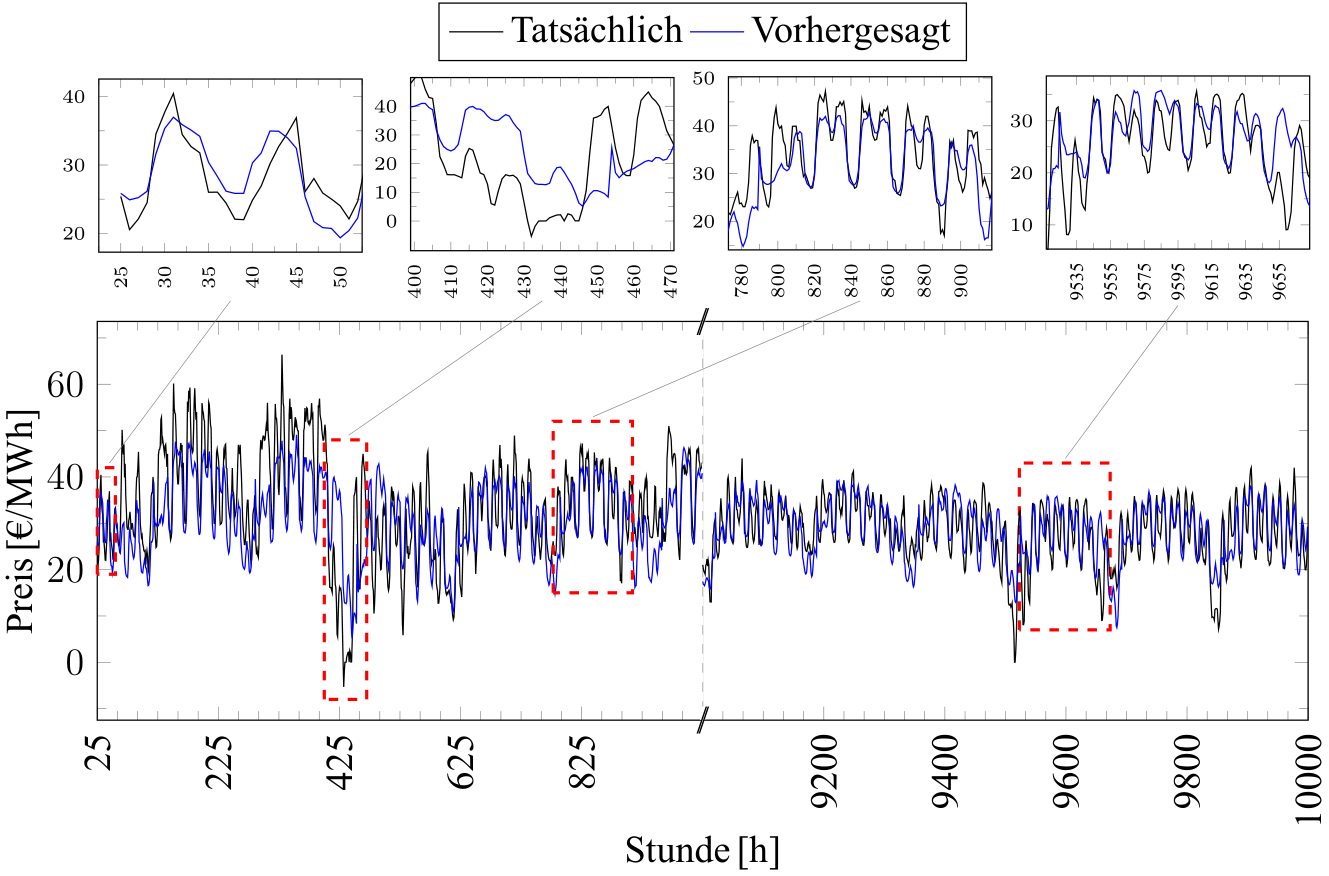
\includegraphics[width=0.92\textwidth]{Bilder/Plot/LM/LM_Preis.PNG}
        %% Compiler: XeLaTeX

\documentclass[tikz,border=0pt]{standalone}%
\usepackage{pgfplots,tikz,color,amsmath,amssymb}
\pgfplotsset{compat=newest}

%\usetikzlibrary{pgfplots.groupplots}
%%-------------------------------------------------------------------------
%% Quellen:
%% Discontinuity: http://www.yesterdayscoffee.de/tag/tikz/
%% https://tex.stackexchange.com/questions/149081/collapse-range-in-x-axis-with-pgfplots-break-x-axis
%% http://guido.vonrudorff.de/pgfplots-discontinuities/





\begin{document}
\makeatletter
\def\datafile{Daten/LM/logist/o/LM_logis_result.txt}
\makeatother

    \pgfplotsset{
        minor x tick num=5,
        minor y tick num=1,
        x label style={yshift=.5em},
        y label style={yshift=-.5em},
        width=15cm,
        height=6cm,
        xticklabel style={
             rotate=90,
        },
        every axis legend/.append style={
        at={(0.5,1.03)},
        anchor=south},
    }


%%----------------------result-----------------------%%
\begin{tikzpicture}
\begin{axis}[
ylabel={Preis\,[€/MWh]},
xlabel={Stunde\,[h]},
xmin=25,
xmax=2025,
clip=false,
xticklabels ={25,225,425,625,825,,9200,9400,9600,9800,10000},
xtick       ={25,225,425,625,825,1025,1225,1425,1625,1825,2025},
extra x ticks={1025},
extra x tick style={grid=major, tick style={white, ultra thick}, tick label style={xshift=0cm,yshift=.30cm,rotate=90,}},
extra x tick labels={\color{white}{/}},
legend style={at={(.5,1.8)},anchor=north},
legend columns=-1,
]

\addplot [mark=none,draw=black,restrict x to domain=25:1024,] 
table[
x=index,
y=real,
col sep=tab,
/pgf/number format/read comma as period,
] {\datafile};
\addlegendentry{Tats\"achlich}
\coordinate (unten) at (axis cs:1025,-12.5);
\coordinate (oben) at (axis cs:1025,73.5);
\draw[white, dashed, line width=.5pt] (unten) -- (oben);


\addplot [mark=none,blue,restrict x to domain=25:1024,] 
table[
x=index,
y=predict,
col sep=tab,
/pgf/number format/read comma as period,
] {\datafile};
\addlegendentry{Vorhergesagt}

\coordinate (oben1) at (axis cs:245,102);
\draw[red, dashed, line width=1pt] (axis cs:25,19) rectangle (axis cs:55,42);
\draw[gray, line width=.2pt] (axis cs:45,43) -- (axis cs:245,78);

\coordinate (oben2) at (axis cs:760,101);
\draw[red, dashed, line width=1pt] (axis cs:400,-8) rectangle (axis cs:470,48);
\draw[gray, line width=.2pt] (axis cs:440,49) -- (axis cs:760,78);

\coordinate (oben3) at (axis cs:1285,103);
\draw[red, dashed, line width=1pt] (axis cs:778,15) rectangle (axis cs:909,52);
\draw[gray, line width=.2pt] (axis cs:844,53) -- (axis cs:1285,78);

\coordinate (oben4) at (axis cs:1810,101);
\draw[red, dashed, line width=1pt] (axis cs:1548,7) rectangle (axis cs:1698,43);
\draw[gray, line width=.2pt] (axis cs:1624,44) -- (axis cs:1810,77);

\addplot [mark=none,draw=black,restrict x to domain=1025:2024,] 
table[
x=index,
y=real,
col sep=tab,
/pgf/number format/read comma as period,
] {\datafile};

\addplot [mark=none,blue,restrict x to domain=1025:2024,] 
table[
x=index,
y=predict,
col sep=tab,
/pgf/number format/read comma as period,
] {\datafile};

\end{axis}
\node at (unten)[white,thick] {/};
\node at (unten) {/\!\!/};
\node at (oben)[white,thick] {/};
\node at (oben) {/\!\!/};

\node at (oben1) {%
    \begin{tikzpicture}[baseline,trim axis left,trim axis right]
    \begin{axis}[
      tiny,
      width=4.5cm, height=3.5cm,
      minor x tick num=1,
      minor y tick num=1,
      xmin=25,xmax=50,
      ytick       ={20,30,40},
      enlargelimits,
    ]
    \addplot +[mark=none,black,] table [x=index,y=real,col sep=tab,/pgf/number format/read comma as period,] {\datafile};
    \addplot +[mark=none,blue,] table [x=index,y=predict,col sep=tab,/pgf/number format/read comma as period,] {\datafile};
    \end{axis}
    \end{tikzpicture}%
    };

\node at (oben2) {%
    \begin{tikzpicture}[baseline,trim axis left,trim axis right]
    \begin{axis}[
      tiny,
      width=4.5cm, height=3.5cm,
      minor x tick num=1,
      minor y tick num=1,
      xmin=405,xmax=465,
      ytick       ={0,10,20,30,40},
      enlargelimits,
    ]
    \addplot +[mark=none,black,] table [x=index,y=real,col sep=tab,/pgf/number format/read comma as period,] {\datafile};
    \addplot +[mark=none,blue,] table [x=index,y=predict,col sep=tab,/pgf/number format/read comma as period,] {\datafile};
    \end{axis}
    \end{tikzpicture}%
    };

\node at (oben3) {%
    \begin{tikzpicture}[baseline,trim axis left,trim axis right]
    \begin{axis}[
      tiny,
      width=4.5cm, height=3.5cm,
      minor x tick num=1,
      minor y tick num=1,
      xmin=785,xmax=905,
      enlargelimits,
    ]
    \addplot +[mark=none,black,] table [x=index,y=real,col sep=tab,/pgf/number format/read comma as period,] {\datafile};
    \addplot +[mark=none,blue,] table [x=index,y=predict,col sep=tab,/pgf/number format/read comma as period,] {\datafile};
    \end{axis}
    \end{tikzpicture}%
    };

\node at (oben4) {%
    \begin{tikzpicture}[baseline,trim axis left,trim axis right]
    \begin{axis}[
      tiny,
      width=4.5cm, height=3.5cm,
      minor x tick num=1,
      minor y tick num=1,
      xticklabels ={9535,9555,9575,9595,9615,9635,9655},
      xtick       ={1560,1580,1600,1620,1640,1660,1680},
      xmin=1555,xmax=1685,
      enlargelimits,
    ]
    \addplot +[mark=none,black,] table [x=index,y=real,col sep=tab,/pgf/number format/read comma as period,] {\datafile};
    \addplot +[mark=none,blue,] table [x=index,y=predict,col sep=tab,/pgf/number format/read comma as period,] {\datafile};
    \end{axis}
    \end{tikzpicture}%
    };
\end{tikzpicture}
\end{document}
    \caption[Gegenüberstellung des tatsächlichen und des vorhergesagten Preises beim LM]{Gegenüberstellung des tatsächlichen und des vorhergesagten Preises, unter Anwendung des Levenberg-Marquardt Algorithmus. Dargestelt ist das MLP mit logistischer Aktivierungsfunktion, ohne Bias-Neuronen und einem $RMSE$-Wert von 7,95.}
    \label{fig:LM_logis_o_result}
\end{figure}

Zu Beginn der Prognose liegt der vorhergesagte nah an dem tatsächlichen Preis, wobei, wie in dem 1. Graphen zu erkennen ist, der maximale Preisunterschied in den ersten 50 Stunden bei circa 10\,€/MWh liegt. Im 3. Graphen lässt sich erkennen, dass das Netzwerk im moderat ausgeprägten Wochenverlauf zwar sehr nah an die negativen Spitzen im Preisverlauf kommt, bei den positiven aber zur Unterschätzung neigt. Wobei extreme Preisänderungen auch bei diesem Lernalgorithmus zu schlechteren Prognosen führen, wie die Preisverläufe des 2. Graphen zeigen, in dem die größte Preisdifferenz bei 30\,€/MWh liegt. Am Ende des Testsets, wie im 4. Graphen zu sehen ist, weist die Prognose neben geringen Abweichungen vom tatsächlichen Preis auch entgegenläufige Preisentwicklungen auf. 

Abschließend erfolgt die Bewertung des Vorhersagevermögens des Netzwerkes anhand der zuvor ausgewählten Performancemaße. Diese sind in \autoref{tab:LM_schaetzer} aufgeführt.

\begin{filecontents*}{LM_resultat.tex}
{\setstretch{1.0}
\captionsetup{skip=1pt,margin=5pt,position=below} %skip=1pt,
\rowcolors{3}{tableShade}{white}

\begin{longtable}{cccccccc}
    %\captionsetup{justification=centering}
    \caption[Übersicht der Performancemaße des genauesten Netzwerkes beim LM-Alg.]{Übersicht der Performancemaße des MLP mit logistischer Aktivierungsfunktion und ohne Bias-Neuronen.} \label{tab:LM_schaetzer}\\
    \toprule
    \hiderowcolors
        $RMSE$ & $MAE$ & $ABS$ & $REL$ & $R^2$ & $RAE$ & $MAPE_2$ & $sMAPE$ \\
    \midrule
    \endfirsthead
        \multicolumn{8}{c}{\footnotesize \tablename\ \thetable{}: Fortsetzung der vorherigen Seite} \\
    \toprule
        $RMSE$ & $MAE$ & $ABS$ & $REL$ & $R^2$ & $RAE$ & $MAPE_2$ & $sMAPE$ \\
    \midrule
    \endhead
    \midrule
        \multicolumn{8}{c}{{\footnotesize \tablename\ \thetable{}: Fortsetzung auf der nächsten Seite}} \\
    \bottomrule
    \endfoot
    \bottomrule
    \endlastfoot
    \showrowcolors
        7,946 & 5,694 & 0,804 & 0,028 & 0,775 & 40,483 & 19,9 & 22,95 \\
\end{longtable}

}
\end{filecontents*}
\LTXtable{\textwidth}{LM_resultat}

Der $ABS$ und der $REL$-Wert sind beide positiv und zeigen somit, dass die Gesamtschätzung eine überschätzte Prognose aufweist. Das $R^2$ besitzt mit 0,775 einen positiven Wert der näher an der 1 als an 0,5 ist und der $RAE$-Wert ist mit 40,483 deutlich unter 100. Hiermit weist das Netzwerk eine höhere Vorhersagegenauigkeit auf als der historische Mittelwert. Die Interpretation der restlichen Schätzer erfolgt im anschließenden Abschnitt.



Bei der Auswertung der Messungen ist aufgefallen, dass der implementierte LM-Algorithmus in einigen Fällen optimale Fehlerwerte ausgibt (ergo einen $RMSE$-Wert von Null usw.). Dies führte bei der Mittelwertbildung der Fehler zu verzerrten Ergebnissen. Nach Bekanntwerden dieser Problematik konnte festgestellt werden, dass hin und wieder nach dem Training die Gewichtsmatrizen des Netzwerkes leer sind. Da die restlichen Ergebnisse aber plausible Werte liefern, wurde von einer Neuprogrammierung abgesehen und die Fehlermittelwerte an die veränderte Anzahl an Ergebnissen angepasst. Das Programm wurde soweit modifiziert, dass falls das Netzwerk nach dem Training leere Gewichte aufweist es neuinitialisiert wird.

\newpage

\subsection{Gegenüberstellung der Analyseergebnisse}\label{sec:geg_aus_alg}

Unter Berücksichtigung der Ergebnisse beider Analysen erfolgt nun eine Gegenüberstellung. Im Hinblick auf die Variation der Aktivierungsfunktion weist die logistische Funktion beim BP-Verfahren höhere Optimierungszeiten auf als mit dem Tangens-Hyperbolicus. Bei der Berechnungszeit und dem $RMSE$-Wert sind jedoch geringere Werte zu beobachten. Aus diesem Grund ist die logistische Funktion beim BP-Verfahren und der betrachteten Anwendung zu bevorzugen.
Die unterschiedlichen Ergebnisse bei Variation der Aktivierungsfunktionen im LM-Algorithmus lassen keine Empfehlung für eine der betrachteten Funktionen zu.\par\medskip

Der Einsatz von Bias-Neuronen führte beim BP-Verfahren zu einer längeren Optimierungs- und Berechnungszeit. Der $RMSE$-Wert fiel mit Bias-Neuronen bei beiden Aktivierungsfunktionen höher aus als ohne diese. Somit führt der Einsatz von Bias-Neuronen nicht zu einer besseren Vorhersage, dafür zu einer längeren Berechnungszeit und ist beim Einsatz des BP-Verfahrens nicht zu empfehlen. Betrachtet man die Optimierungszeit als Maß für die Trainingszeit, so kann die Aussage, dass Bias-Neurone zu schnellerem Lernen führen, nicht bestätigt werden.
Beim LM-Algorithmus führt der Einsatz von Bias-Neuronen zwar ebenfalls zu einer längeren Optimierungszeit, jedoch kann die Berechnungszeit mit Bias-Neuronen auch kürzer ausfallen als ohne diese.\par\medskip 

Die Optimierungszeit der untersuchten Netzwerkkonstellationen betrug beim BP-Verfahren zwischen 6h:46m:50s und 8h:29m:29s. Beim LM Algorithmus lag die Optimierungszeit zwischen 4h:52m:11s und 11h:29m:02s. Betrachtet man die Optimierungszeiten ohne Bias-Neuronen, so liegt diese beim BP-Verfahren zwischen 6h:46m:50s und 7h:44m:39s und beim LM-Algorithmus zwischen 4h:52m:11s und 5h:05m:04s womit der LM-Algorithmus weniger Optimierungszeit benötigt. Bei der Berechnungszeit weist das BP-Verfahren Werte zwischen 10s-16s auf. Im Vergleich zeigt der LM-Algorithmus Werte zwischen 7m:10s-19m:16s. Dieser Unterschied kann einerseits durch die unterschiedliche Anzahl an verdeckten Neuronen begründet sein. Die Anzahl verdeckter Neuronen fällt beim BP-Verfahren mit 3-5 niedriger aus, als beim LM-Algorithmus mit 10-13. Andererseits sucht der LM-Algorithmus bei jeder Berechnung aufs Neue die optimalen Parameter und besitzt dadurch zwar eine kürzere \glqq manuelle\grqq~Optimierungszeit, aber auch eine längere Berechnungszeit. Das BP-Verfahren benötigt mehr Zeit bei der Optimierung aber nachdem die optimalen Parameter für den Datensatz gefunden sind, können sie bei jeder Prognose genutzt werden, wodurch sich die Berechnungszeit verkürzt.\par\medskip

Die Abweichung des $RMSE$ sowie des $MAE$-Schätzers zwischen den beiden Lernalgorithmen beträgt 0,361 und 0,486 respektive, wobei Der LM-Algorithmus jeweils den geringeren Wert aufweist. Die Differenz des $MAPE$ und des $sMAPE$ beträgt 1,697 und 3,091, wobei ebenfalls der LM-Algorithmus den geringeren Wert besitzt. Somit weist der LM-Algorithmus eine geringfügig bessere Prognose auf als das BP-Verfahren. Da bei beiden Algorithmen die Gewichte zu Beginn des Trainings zufällig gewählt werden, weisen die geringen Abweichungen eher auf ungünstige Minima in der Fehlerlandschaft als auf bessere Prognosefähigkeiten des LM-Algorithmus hin.\par\medskip

Demnach ist das Backpropagation-Verfahren bei gleichbleibendem Datensatz zu bevorzugen. Wohingegen der Levenberg-Marquardt Algorithmus bei Untersuchungen mit wechselnden Datensätzen zu schnelleren Ergebnissen führt.


